\chapter{Deseño e Implementación}

Neste capítulo veremos detalles do deseño e implementación de diferentes partes do programa.

\section{Módulo de Ficheiros}

O módulo de xestión de ficheiros é un do máis importantes e complexos de todo o programa, o cal é lóxico tendo en conta que o programa é un editor de ficheiros.

En canto ao deseño, ó principal obxectivo é a estensibilidade do mesmo pois, aínda que o programa está centrado na edición de ficheiros PO e son estes os únicos soportados na actualidade, preténdese que o programa sexa capaz de soportar varios tipos de ficheiros nun futuro. Na figura~\ref{fig:dia_class:files} pódese ver o diagrama de clases deste módulo.

\subsection{Implementación Xenérica}
A implementación da clase \lstinline{File} contén propiedades para conseguir información sobre o nome e \emph{path} onde está dito ficheiro, ademais garda estatísticas sobre o número de mensaxes traducidos, sen traducir ou con tradución difusa. Estas estatísticas actualízanse cada vez que se engade ou elimina unha cadea ou cada vez que esta se modifica. Tamén contén un valor booleano que permite saber se o ficheiro foi modificado. Aparte de métodos para engadir e eliminar cadeas, e para conseguir e modificar os metadatos do ficheiro esta clase ten un método para gardar e recuperar o ficheiro. O método para gardar~(\lstinline{save}) emprega o patrón \emph{Template Method}\cite{book:gang4pat} o cal nos permíte actualizar o estado do ficheiro a non modificado.

Un ficheiro contén instancias de mensaxes~(\lstinline{Message}). As mensaxes teñen como propiedades un estado, orixes, e consellos. A API prové métodos para conseguir e modificar tanto as cadeas orixinais como as traducións, na súa forma en singular ou nalgunha das formas plurais. A implementación do método para modificar unha tradución tamén emprega o patrón Template Method para actualizar o estado da mensaxe. Esta clase tamén ten métodos para engadir e eliminar consellos e para obter o contexto da mensaxe.

\begin{figure}[h!]
    \centering
    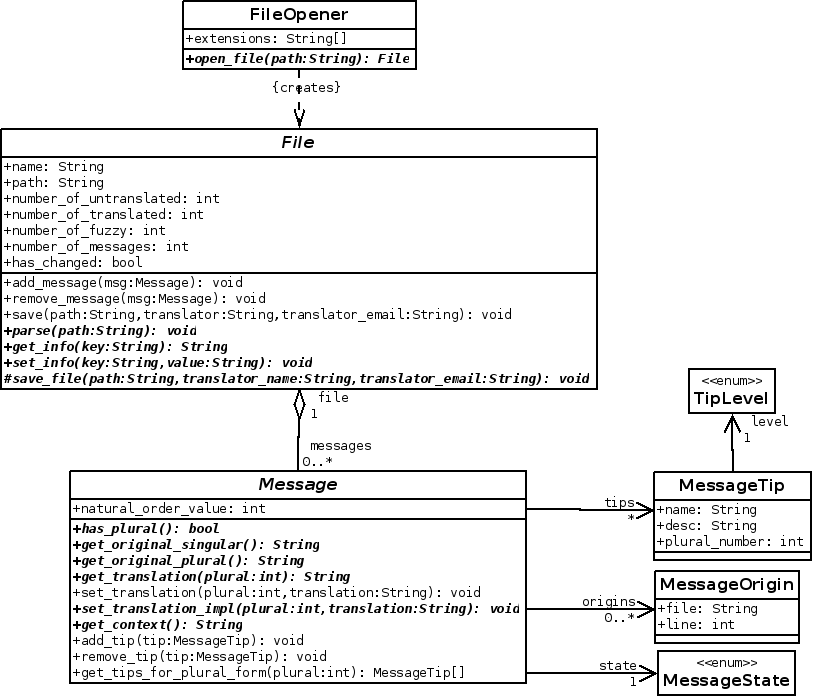
\includegraphics[width=\textwidth]{img/genericfile.png}
    \caption{Diagrama de Clases do módulo ficheiros}
    \label{fig:dia_class:files}
\end{figure}

Ademais a clase \lstinline{FileOpener} recolle un método para crear ficheiros e un conxunto de extensións que se poden abrir con este FileOpener.

\subsubsection{Consellos (Tips)}
Os consellos son a solución que damos para aportar información ao usuario sobre a tradución que está a realizar. Algunhas das cousas que poden axudar a indicar esta característica son se a tradución está a ser demasiado longa, se hai algunha palabra que está mal escrita na tradución ou se non emprega a terminoloxía adecuada.

Cada consello ten un nome que debe ser xenérico a cada clase de consello, unha descrición que ten que explicar o problema con detalle, un nivel que indica a gravidade do consello e unha referencia a forma plural a que corresponde dito consello. Ademais, pode conter unha ou máis referencias á localización exacta do problema que permitirá destacala na interface gráfica.

A creación de consellos farase ó modificarse unha cadea e farase a través de plugins.

\subsubsection{Pistas (Hints)}
As pistas amosaranlle ó usuario posibles traducións ou aproximacións ás traducións. Estas pistas poden ser obtidas de memorias de traducións, de traducións do mesmo ficheiro noutra linguaxe, ou da tradución directa, por exemplo.

Cada instancia dunha pista~(\lstinline{Hint}) contén a tradución suxerida, unha cadea que identifica a orixe de dita pista e un valor que indica a precisión de dita suxerencia.

De igual forma que no caso dos consellos a creación de pistas correrá ó cargo de plugins creados a tal propósito. Neste caso actualizaranse as pistas de cada mensaxe ao seleccionalo mesmo na interface.

\subsection{Ficheiro PO}
A implementación específica para ficheiros PO (Figura~\ref{fig:dia_class:pofile}) estende as clases \lstinline{File}, \lstinline{FileOpener} e \lstinline{Message} abstractas para implementar os métodos e permitir empregar ficheiros PO.

Para a análise e a actualización dos ficheiros PO empregaremos a biblioteca gettext-po. No momento no que se iniciou a implementación deste módulo, non existía implementación desta librería en Vala polo que tivemos que crear uns \emph{bindings} para poder empregala.

Tanto a clase PoFile como a clase PoMessage delegan a maior parte dos seus métodos nas instancias das clases dos bindings da biblioteca GettextPo File e Message respectivamente. Desta forma faise un claro uso do patrón \emph{Adapter}\cite{book:gang4pat}.

\begin{figure}[h!]
    \centering
    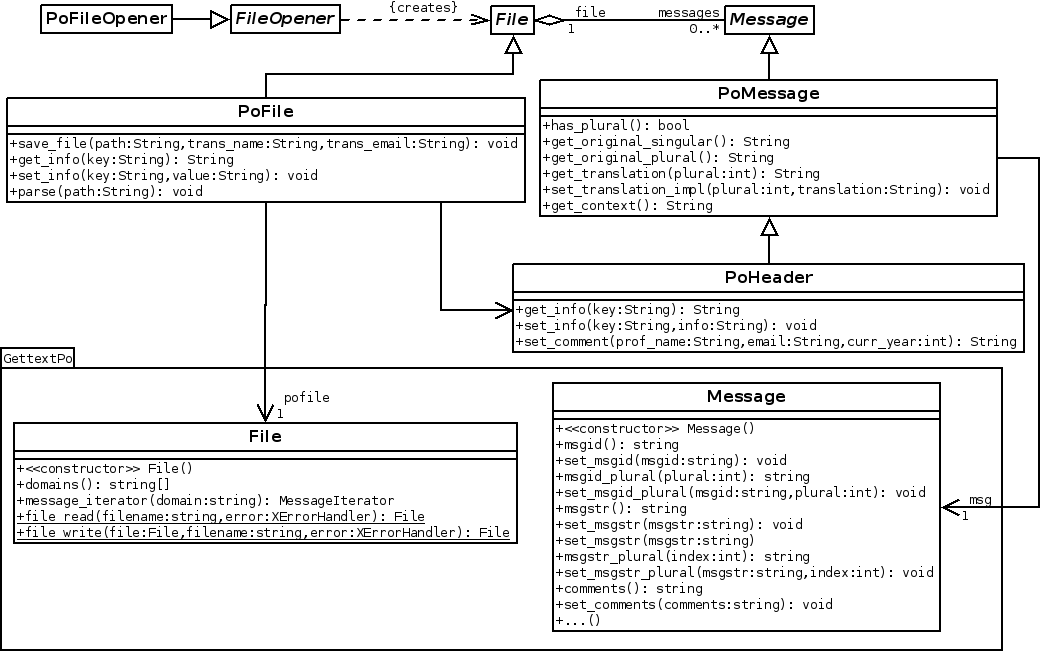
\includegraphics[width=\textwidth]{img/pofile.png}
    \caption{Diagrama de Clases do ficheiro PO}
    \label{fig:dia_class:pofile}
\end{figure}

De forma adicional, a clase PoFile contén unha instancia da clase PoHeader. Esta clase que estende a PoMessage ten os metadatos que se atopan nos ficheiros PO na tradución da cadea baleira. Ademais, esta, dipón de métodos para obter e modificar metadatos e para actualizar os datos dos autores das traducións de dito ficheiro. A clase PoFile delega nesta clase á hora de conseguir e modificar metadatos e tamén cando garda un ficheiro.

A clase \lstinline{PoFileOpener} só é capaz de abrir ficheiros con estensión PO e simplemente emprega o método parse da clase ficheiro para crear unha nova instancia.

\subsubsection{Implementación dos bindings}
Como xa mencionamos vímonos na obriga de crear nós os bindings para a biblioteca gettext-po. Vala é unha linguaxe deseñada para permitir o fácil acceso a outras bibliotecas escritas en C, especialmente se se trata de bibliotecas baseadas en GObject. Despois de todo Vala emprega C como linguaxe intermedio. A biblioteca gettext-po non é unha biblioteca baseada en GObject polo que a creación destes bindings é un pouco máis complicado.

Para poder empregar unha biblioteca escrita en C no noso programa escrito en Vala só temos que crear un ficheiro con extensión VAPI que conteña en sintaxe Vala as clases da biblioteca engadindo unhas etiquetas que permitan a súa tradución ó código C correcto. No Fragmento de código~\ref{lst:bindingsgettext} podemos ver parte dos bindings creados para a biblioteca gettextpo.

\lstset{language=[sharp]C}
\begin{lstlisting}[label=lst:bindingsgettext,caption=Bindings da biblioteca GettextPo]
[CCode (cprefix = "Po", lower_case_cprefix = "po_")]
namespace GettextPo {

    [CCode(cheader_filename = "gettext-po.h", cname="struct po_file", free_function="po_file_free")]
    [Compact]
    public class File {

        [CCode (CCode = "po_file_create")]
        public File();

        [CCode (array_length = false, array_null_terminated = true, cname="po_file_domains")]
        public unowned string[] domains ();

        [CCode (cname="po_file_write")]
        public static unowned GettextPo.File file_write (GettextPo.File file,
                            string filename,
                            XErrorHandler handler);
        [...]
    }

    [CCode(cheader_filename = "gettext-po.h", cname="struct po_message")]
    [Compact]
    public class Message  {

        [CCode (cname="po_message_create")]
        public Message();
        public unowned string msgid ();
        public unowned string? msgid_plural ();
        [...]
\end{lstlisting}

Como podemos ver, o traballo practicamente limítase a establecer o parámetro \lstinline{cname} en cada clase e método. Hai que ter en conta que non sempre é necesario especificar este parámetro pois as bibliotecas empregan case sempre unhas normas de nomeado que fan que usen primeiro o nome da biblioteca, despois o nome da clase e logo o nome do método separado por barras baixas. Desta forma no método da biblioteca \lstinline{po_message_msgid()}, \emph{po\_} corresponde o nome da biblioteca, \emph{message\_} ao nome da clase e \emph{msgid} ao nome do método. Os bingings de Vala empregan estas normas para nomear os métodos polo que, en ocasións, non é necesario especificar o parámetro \lstinline{cname}. Isto sucede, como se pode ver no Fragmento de código~\ref{lst:bindingsgettext}, no caso da clase Mensaxe (\lstinline{Message}).

Ademais, é necesario especificar o nome do ficheiro cabeceira que se emprega e no caso de que o tipo de retorno sexa un array temos que especificar máis parámetros, como acontece no método \lstinline{domains()} da clase File. Por último, é importe especificar a pertenza de cada valor e os métodos correctos para liberar as instancias, desta forma evitaremos que haxa perdas de memoria e fallos de segmentación.

\section{Módulo de Linguaxes}
O módulo de linguaxes xestiona os linguaxes e formas plurais existentes. Contén dúas clases, a clase \lstinline{Language} e a clase \lstinline{PluralForm}. Estas dúas clases provén un método estático para obter as instancias existentes. Estas instancias créanse a primeira vez que se carga a clase consultando unhas bases de datos que consisten nuns ficheiros JSON\footnote{\href{http://gl.wikipedia.org/wiki/JSON}{JSON}}.

\begin{figure}[h!]
    \centering
    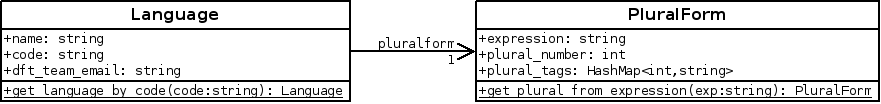
\includegraphics[width=\textwidth]{img/languages.png}
    \caption{Diagrama de Clases do módulo de Linguaxes}
    \label{fig:dia_class:languages}
\end{figure}

Como podemos ver na Figura~\ref{fig:dia_class:languages}, en cada instancia dunha linguaxe contén o nome da linguaxe, o seu código empregando a norma ISO 639-1, a súa forma plural e o email do equipo de tradución por defecto. Engadimos o idioma do equipo de tradución por defecto para autocompletar este campo no perfil do usuario. No Fragmento de Código~\ref{lst:languages} podemos ver un fragmento do ficheiro JSON contendo as linguaxes.

\begin{lstlisting}[label=lst:languages,caption=Fragmento da Base de Datos de Linguaxes]
  {
    "languages" : [
      [...]
      {
        "code" : "es",
        "name" : "Spanish; Castilian",
        "pluralform" : "nplurals=2; plural=(n != 1);",
        "default-team-email": "gnome-es-list@gnome.org"
      },
      [...]
    ]
  }
\end{lstlisting}

En canto á clase \lstinline{PluralForm}, esta clase inclúe o número de plurais, a expresión desa forma plural e un conxunto de etiquetas. Estas etiquetas pretenden facilitar ó usuario a identificación de que número corresponde a cada forma plural. No Fragmento de Código~\ref{lst:plurals} pódemos ver unha parte da base de datos de formas plurais.

\begin{lstlisting}[label=lst:plurals,caption=Fragmento da Base de Datos de Plurais]
  {
    "forms" : [
      {
        "expression" : "nplurals=2; plural=(n > 1);",
        "number_of_plurals" : 2,
        "tags" : [
          {
            "number" : 0,
            "tag" : "Equal to 0 or 1"
          },
          {
            "number" : 1,
            "tag" : "Greater than 1"
          }
        ]
      },
      [...]
    ]
  }
\end{lstlisting}

\section{Interface Gráfica}
A interface gráfica é unha das partes á que máis tempo lle dedicamos neste proxecto. O obxectivo dende o principio foi construír algo simple pero potente que permitira ó usuario editar os ficheiros PO de forma sinxela, pero que fose capaz de aportarlle moita información que lle axudase a facer a tradución.

\subsection{Evolución}
Durante a execución do proxecto probamos diferentes formas da interface gráfica ata chegar ó resultado actual. Estas versións pretenden imitar programas existenttes e obedecen xeralmente a conversacións con tradutores.

\subsubsection{Primeira Versión: moi semellante a GTranslator}
Para comezar a traballar, e tras amosar varios mockups nos reportes recibindo feedback sobre eles, decidimos facer unha interface de usuario moi parecida a de GTranslator. Esta interface inclúe bloques para a lista de mensaxes, editar ditos mensaxes e amosar o contexto. Estes bloques pódense mover por toda a interface e incluso separar da mesma xa que estamos empregando a biblioteca GNOME Docking Library. Na Figura~\ref{fig:ui:v1:general} podemos ver, o aspecto desta primeira versión da interface.

\begin{figure}[h!]
  \centering
    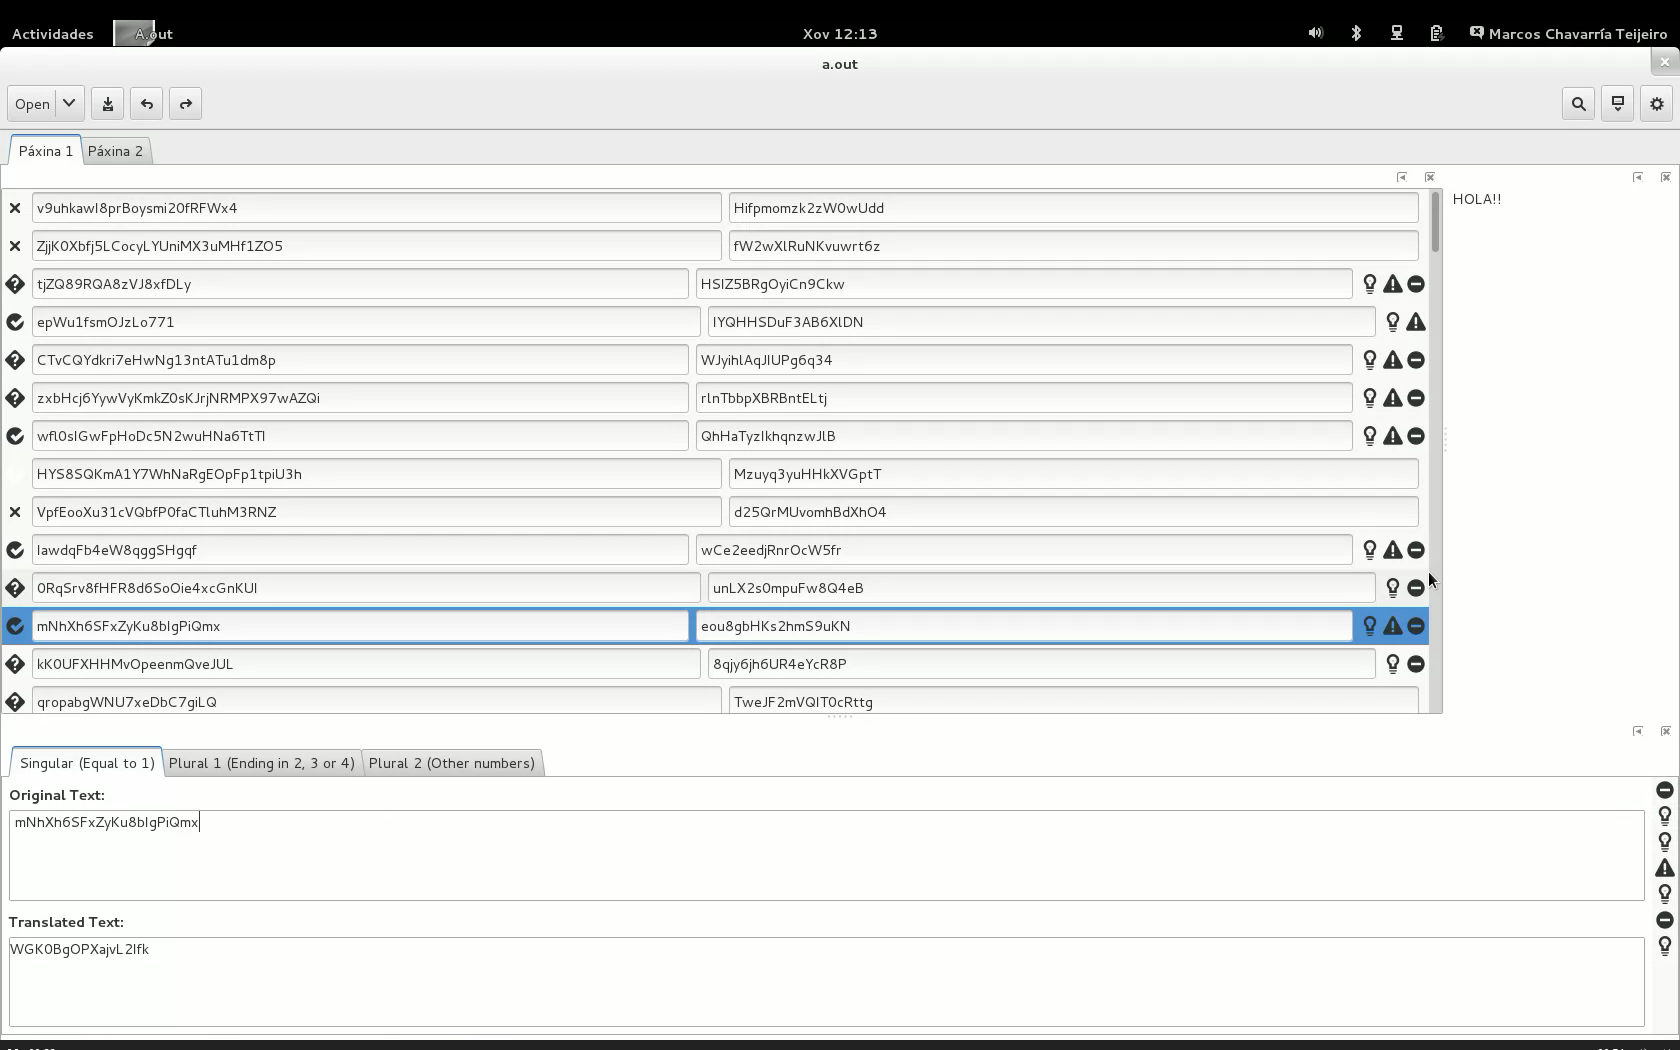
\includegraphics[width=\textwidth]{img/gsoc1_it2_ui.png}
    \caption{Primeira versión da interface de usuario}
    \label{fig:ui:v1:general}
\end{figure}

Como podemos ver a interface contén un barra de ferramentas que permite abrir ficheiros, gardalos, desfacer e refacer cambios, buscar no documento e ver as preferencias. Permite abrir diversos ficheiros en varias lapelas. En cada unha das lapelas podemos ver a lista de mensaxes e o widget de edición.

En cada mensaxe da lista, aparte das cadeas orixinal e traducida, podemos ver o estado da cadea e se está ten consellos (Tips) activos e de o nivel de estes. Por outro lado, no widget de edición podemos ver unha lapela por cada forma plural que podemos editar e unha lista vertical con iconas cos consellos. Ao pasar o rato polo consello veremos a súa descrición.

\begin{figure}[h!]
  \centering
  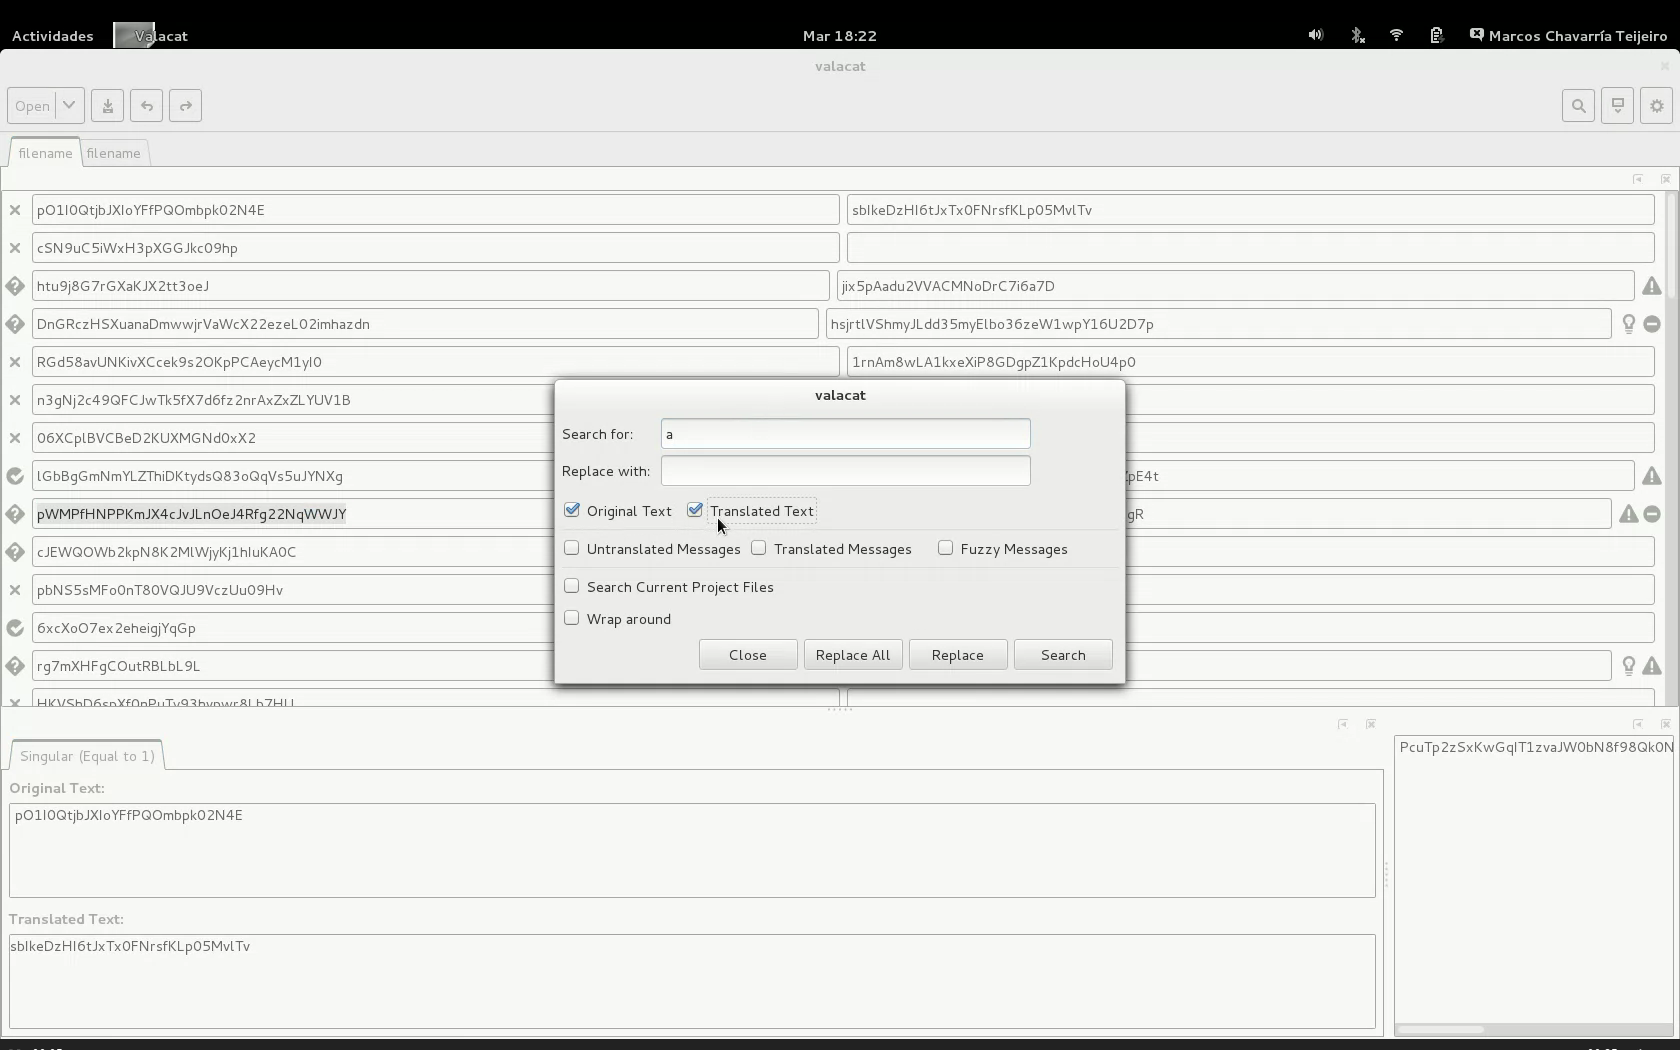
\includegraphics[width=0.4\textwidth]{img/gsoc1_it3_ui.png}
  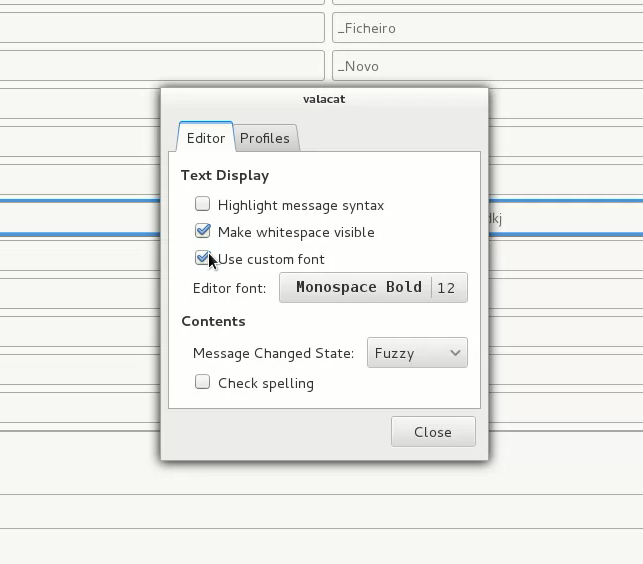
\includegraphics[width=0.4\textwidth]{img/gsoc1_it5_prefs.png}
  \caption{Diálogos da primeira versión da interface de usuario}
  \label{fig:ui:v1:dialogs}
\end{figure}

Como podemos ver na Figura~\ref{fig:ui:v1:dialogs} tanto á hora de xerar unha busca como para ver as preferencias, esta interface empregará uns diálogos non modais.

En conversacións en IRC con tradutores e anteriores mantedores de GTranslator chegamos á conclusión de que o uso de GNOME Docking Library era unha mala idea, pois significaba un erro de deseño xa que, se o usuario tiña que modificar o aspecto da interface, era debido a que o deseño non era correcto. Esta biblioteca, ademais, ten bastantes fallos polo que non era recomendable usala.

Ademais, durante a GUADEC, comentáronos da existencia dun widget moito mellor para xestionar a buscas, consistente nunha barra horizontal que se desplegaba cando a busca estaba activa.

Por outro lado, o resultado deste modelo de interface tampouco era demasiado satisfactorio polo que intentamos probar cunha versión máis próxima ó programa Virtaal.

\subsubsection{Segunda Versión: semellante a Virtaal}

Para lograr un aspecto máis parecido ó da aplicación Virtaal fusionamos o widget de edición e o widget de lista de cadeas.

A aplicación segue mantendo as lapelas que permiten abrir máis dun ficheiro ó mesmo tempo, pero eliminamos a posibilidade de personalizar a interface. En lugar diso crearemos unha interface con dúas columnas, na primeira teremos o widget para listar e editar as cadeas e na segunda un widget para ver o contexto e outro para ver as pistas.

Modificamos a barra de ferramentas que converteremos nun \lstinline{GTK.HeaderBar} que permite fusionar esta barra de ferramentas co marco da ventá. O uso de HeaderBars son un patrón de deseño recomendado por GNOME na súa Guía de Interfaces Humanas (\emph{HIG})\cite{website:gnomehig}. Na Figura~\ref{fig:ui:v2:general} podemos ver como quedou a nova inteface.

\begin{figure}[h!]
  \centering
    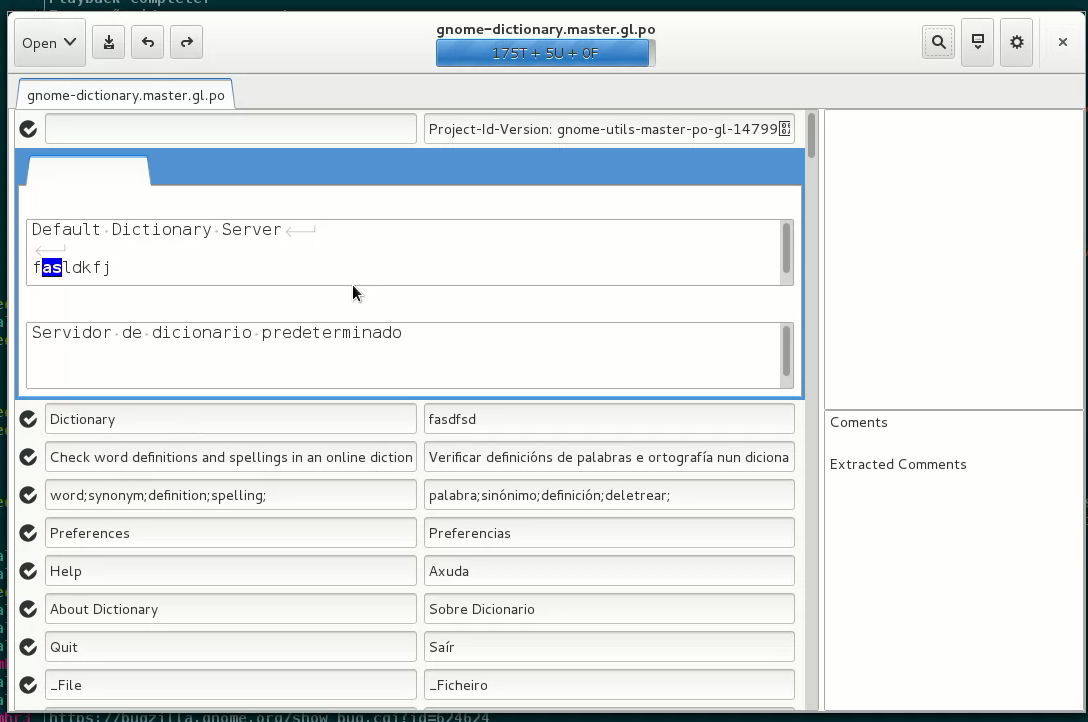
\includegraphics[width=\textwidth]{img/curso2014_it1_ui.png}
    \caption{Segunda versión da interface de usuario}
    \label{fig:ui:v2:general}
\end{figure}

Outro dos aspectos da interface no que se traballou foi na eliminación do diálogo de nova busca. Como se pode ver na Figura~\ref{fig:ui:v2:search}, ó activar a busca, desplégase unha barra horizontal que permite introducir termos para buscar.

\begin{figure}[h!]
  \centering
    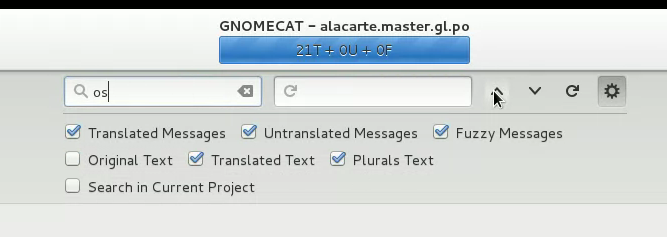
\includegraphics[width=0.8\textwidth]{img/curso2014_it2_search.png}
    \caption{Barra de busca}
    \label{fig:ui:v2:search}
\end{figure}

Para construír esta barra empregamos o widget \lstinline{GTK.SearchBar}. Creamos un modo de busca normal e un modo avanzado. O modo normal amosa unha caixa de texto para introducir a busca e frechas para avanzar na busca, e o modo avanzado engade unha segunda entrada de texto e un botón para a opción de buscar e remplazar e permite seleccionar que cadeas queremos incluír na busca.

Esta interface, aínda que máis pulida cá anterior, presentaba problemas á hora de editar longas cadeas de texto. Ademais, non deixaba demasiado espazo para engadir información sobre as cadeas. Debido a isto escribimos un artigo con algúns mockups baseados en algúns deseños feitos para GTranslator. Durante o GSoC 2014 creamos a que está pensada como a interface definitiva do programa.

\subsubsection{Terceira Versión}
Para a realización desta terceira versión e definitiva intentamos poñernos en contacto cos deseñadores de GNOME para que nos axuden co deseño da nova interface. Ante a baixa participación neste sentido por parte dos deseñadores, usamos uns deseños feitos por Daniel Korostil para un redeseño de GTranslator que nunca chegou a implementarse. Baseándonos nestes mockups e en ideas propias creamos un novo concepto de interface que ten como idea principal a de intentar eliminar onde sexa posible calquera diálogo externo ó programa.

A ventá pasa a compoñerse dunha barra de ferramentas integrada nun \lstinline{GTK.HeaderBar}, unha barra de notificacións e un conxunto de paneis.

\begin{figure}[h!]
  \centering
    
\includegraphics[width=0.8\textwidth]{img/editheaderbar.png}
    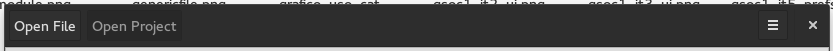
\includegraphics[width=0.8\textwidth]{img/openedfilesheaderbar.png}
    
\includegraphics[width=0.8\textwidth]{img/preferencesheaderbar.png}
    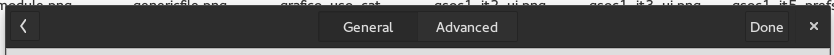
\includegraphics[width=0.8\textwidth]{img/profileheaderbar.png}
    \caption{Diferentes Barras de Ferramentas}
    \label{fig:ui:v3:headerbar}
\end{figure}

A barra de ferramentas é dinámica e os botóns que amosa dependen de que pantalla se estea mostrando no programa. Esta é unha das suxerencias que a Guía de Interfaces Humanas de GNOME fai.

Para lograr isto dentro do \lstinline{GTK.HeaderBar} introducimos un widget denominado \lstinline{GTK.Notebook}. Este widget é o mesmo que se empregaba en versións anterior da interface para ter diferentes ficheiros abertos en outras tantas lapelas, pero empregando a opción que este incorpora de ocultar as lapelas. Desta forma, cada páxina do GTK.Notebook é unha das opcións da barra de ferramentas. Na Figura~\ref{fig:ui:v3:headerbar} podemos ver algúnhas das diferentes formas da barra de ferramentas.

Os botóns da barra de tarefas xeran accións de GTK que serán manexadas pola ventá. A ventá manexará estas accións delegando no panel que esté activo nese momento facendo uso do patrón \emph{State}\cite{book:gang4pat}. No Fragmento de Código~\ref{lst:oneditsave} pódese ver un exemplo da implementación dun dos manexadores.

\lstset{language=[sharp]C}
\begin{lstlisting}[label=lst:oneditsave,caption=Implemenación do manexador da acción gardar]
  private void on_edit_save ()
  {
    (window_panels.get_nth_page (window_panels.page) as Panel).on_edit_save (this);
  }
\end{lstlisting}

Tamén empregamos un GTK.Notebook para cambiar entre paneis. Os paneis son as diferentes pantallas que se poden ver no programa. Desta forma, temos un panel para abrir ficheiros, un panel para as preferencias e un panel para editar os ficheiros entre outros. Na implementación cada panel ten que implementar a interface Panel. Esta interface pide que se defina un tipo de barra de tarefas e dá unha implementación xenérica ós manexadores das accións da ventá. Cada panel será libre de aportar unha implementación especifica destas accións. Na seguinte sección trataranse en detalle cada un dos paneis da interface.

En canto á barra de notificación, é a resposta que damos á necesidade de avisar ó usuario de certos eventos do programa. Por exemplo, avisamos ó usuario que está introducindo unha busca, de que non existe ningunha cadea que cumpra o criterio ou, se este está avanzando polas cadeas, que xa chegou á última. Para implementar esta parte fixemos uso do widget \lstinline{GTK.InfoBar}. Amosamos a notificación durante unha certa cantidade de tempo e despois ocultámolo. Na Figura~\ref{fig:ui:v3:infobar} vemos unha captura da barra de notificación.

\begin{figure}[h!]
  \centering
    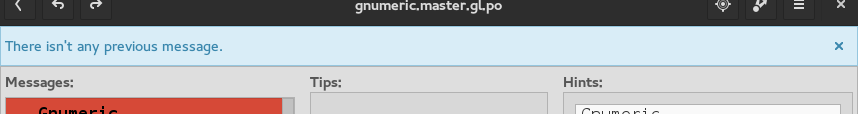
\includegraphics[width=0.7\textwidth]{img/gsoc2_it3_ui.png}
    \caption{Barra de Notificacións}
    \label{fig:ui:v3:infobar}
\end{figure}

Por último, tamén engadimos un menú de aplicación que permite acceder ó panel de preferencias, pechar o programa e iniciar un dialogo para obter información sobre quen fixo GNOMECAT e a súa licenza, entre outros. O uso de menús de aplicación en GNOME é unha recomendación da súa Guía de Interfaces Humanas. Pódese acceder ó menú de aplicación dende GNOME facendo click na icona da aplicación na barra superior do entorno de ventás.

\subsection{Paneis}
Os paneis empregados no programa son os seguintes:

\subsubsection{Panel de Benvida}

O panel de benvida amósaselle ó usuario cando non hai ningún perfil dispoñible no programa. Isto sucede se é a primeira vez que se inicia o programa ou se de forma externa se borrou a información dos perfiles.

\begin{figure}[h!]
    \centering
    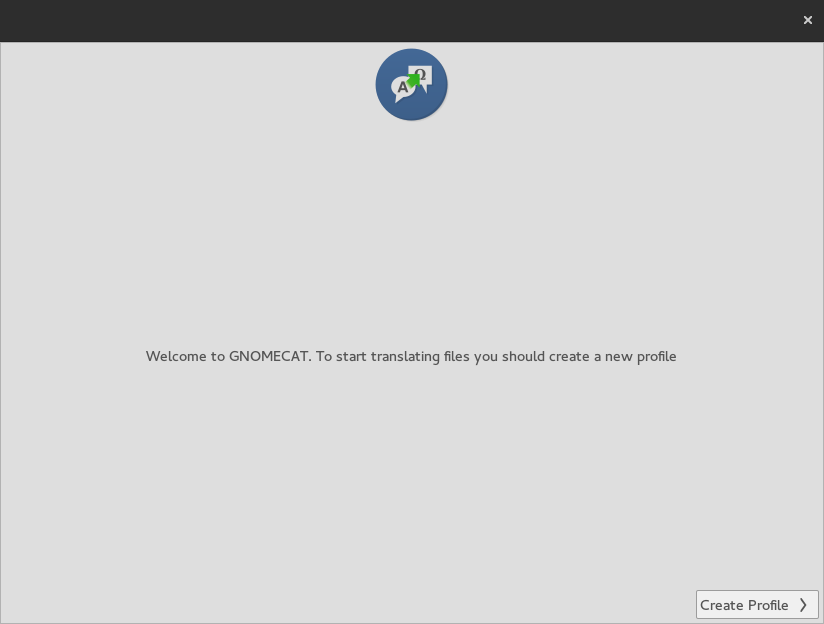
\includegraphics[width=0.8\textwidth]{img/panel_benvida.png}
    \caption{Panel de Benvida}
    \label{fig:ui:panel:welcome}
\end{figure}

Como podemos ver na Figura~\ref{fig:ui:panel:welcome}, amósaselle unha mensaxe de información ó usuario permíndolle acceder ó panel de creación do primeiro perfil.

A barra de ferramentas non inclúe ningún botón xa que a interface só permite avanzar cara ó panel de creación do primeiro perfil ou pechar o programa.

\subsubsection{Panel de ficheiros abertos}

Este panel, como o seu nome indica, amosa unha lista de ficheiros abertos. É o que primeiro se amosa cando abrimos o programa e xa temos perfil creado. Ademais, permite abrir novos ficheiros.

\begin{figure}[h!]
    \centering
    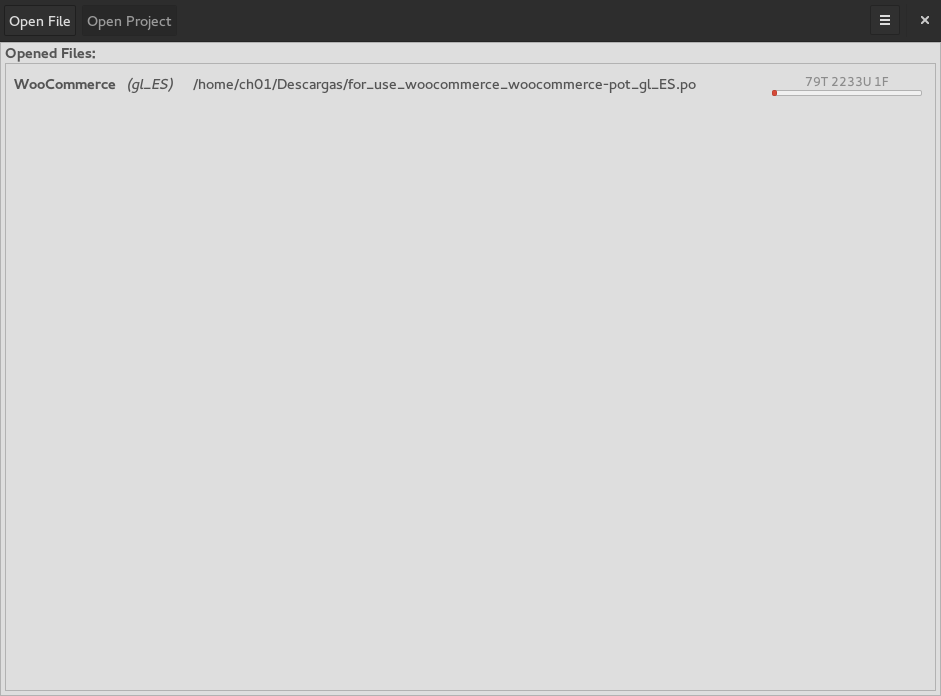
\includegraphics[width=0.8\textwidth]{img/panel_ficheiros_abertos.png}
    \caption{Panel de Ficheiros Abertos}
    \label{fig:ui:panel:openedfiles}
\end{figure}

Na Figura~\ref{fig:ui:panel:openedfiles} pódese ver este panel. Para cada un dos ficheiros abertos amosamos o nome do proxecto segundo aparece nos metadatos do ficheiro PO; a linguaxe deste ficheiro, o path absoluto onde este se atopa e as estatísticas de tradución.

Ademais de permitir abrir un novo ficheiro, a barra de ferramentas tamén permite acceder ó panel de preferencias.

\subsubsection{Panel de abrir ficheiro}

O panel de abrir ficheiros amosa os ficheiros abertos de forma recente e permite abrir novos ficheiros.

Para poder implementar a lista de ficheiros recentes tivemos que crear un widget personalizado. O novo widget emprega a clase \lstinline{GTK.RecentManager}. Esta clase, que funciona empregando o patrón \emph{Singleton}\cite{book:gang4pat}, controla os ficheiros que se abren en todo os sistema. O widget creado conectase á instancia de RecentManager para modificar a lista de ficheiros recentes cada vez que un ficheiro compatible é aberto.

A hora de amosar a información sobre os ficheiros amosamos os mesmos campos que no caso do panel de ficheiros abertos. Isto é debido a que nos dous casos empregamos un GTK.ListBox ao que lle introducimos un widget PoFileRow por cada un dos ficheiros.

\begin{figure}[h!]
  \centering
    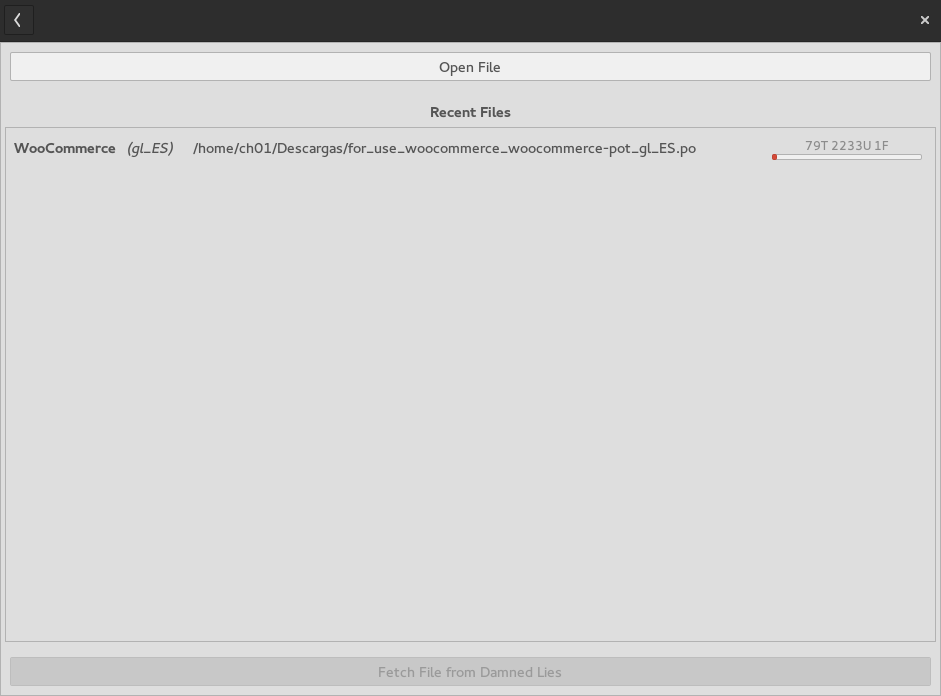
\includegraphics[width=0.8\textwidth]{img/panel_abrir_ficheiro.png}
    \caption{Panel de Abrir Ficheiro}
    \label{fig:ui:panel:openfile}
\end{figure}

Como podemos ver na Figura~\ref{fig:ui:panel:openfile} a barra de ferramentas permite volver a último panel que neste caso sempre será o panel de ficheiros abertos.

\subsubsection{Panel de edición}

O panel de edición é o máis importante deste programa e ao que lle dedicamos máis tempo. Como os seu nome indica permite editar os ficheiros. Está composto de tres columnas, unha lista de mensaxes, unha lista de pistas e unha columna central que contén os consellos, entradas para editar as cadeas e o contexto. As columnas que teñen a lista de mensaxes e de pistas teñen un ancho fixo e a columna central aproveitará todo o espazo restante.

\begin{figure}[hp!]
    \centering
    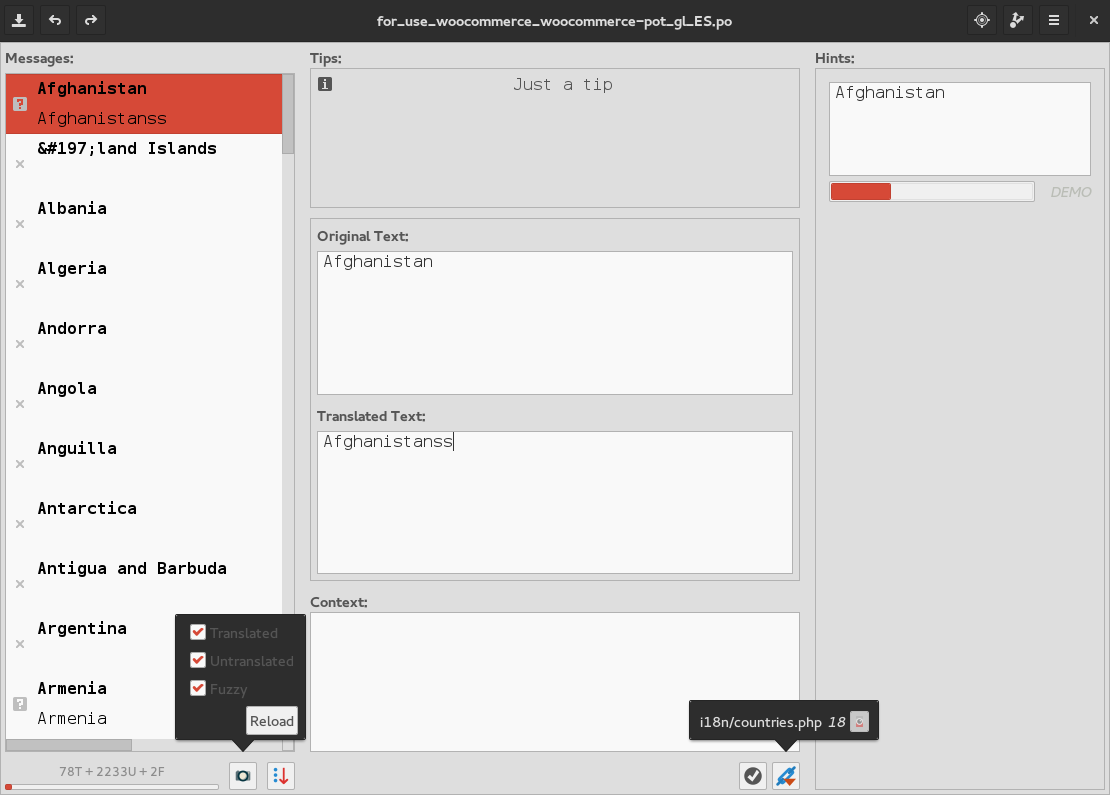
\includegraphics[angle=90,width=\textwidth]{img/panel_edicion.png}
    \caption{Panel de Edición de Ficheiros}
    \label{fig:ui:panel:edit}
\end{figure}

Como se pode comprobar nesta versión da interface, as caixas de edición de cadeas son considerablemente máis grandes que nas outras versións. Na Figura~\ref{fig:ui:panel:edit} podemos ver unha captura deste panel.

A parte que máis traballo nos supuxo foi implementar a lista de mensaxes. Inicialmente deseñamos este \emph{widget} como un \lstinline{GTK.ListBox} coas súas columnas. Este é un widget engadido na versión 3.10 de GTK+ e que empregamos moito no noso programa. A vantaxe de empregalo consiste en que é moi sinxelo personalizar cada columna e aínda que non o usamos no noso programa existiría a posibilidade de engadir columnas de diferentes tipos. O problema que atopamos cando construímos o widget de listar mensaxes con un \lstinline{ListBox} é que este funcionaba realmente mal cando o ficheiro tiña moitas cadeas. Primeiro pensamos que a lentitude debíase ao alto consumo de memoria cando cargabamos un destes ficheiros pero máis tarde falando con algún desenvolvedor de GTK+, démonos conta de que este widget non estaba deseñado para soportar tantas columnas e que debíamos empregar unha alternativa.

A alternativa escollida foi a de empregar un \lstinline{GTK.TreeView}. Este widget si que esta deseñado para soportar gran cantidade de columnas pero a personalización de cada columna e moito máis complicada. Para facelo tivemos que implementar un \lstinline{GTK.CellRenderer} para o renderizado das columnas. Nesta clase especificamos a man onde se debuxa cada elemento da columna e que tamaño ten.

A clase \lstinline{TreeView} incorpora métodos que permiten ordenar e filtrar de forma sinxela as columnas que se amosan neste widget. Isto permitiunos engadir estas opción a nosa interface. Como se pode ver na figura anterior debaixo da lista de mensaxe temos unha barra coas estatísticas do documento e dous botóns un permite filtrar os resultados ocultando ou amosando as cadeas traducidas, sen traducir ou con tradución difusa e o outro permite ordenar as mensaxes amosando primeiro as mensaxes sen traducir, despois as mensaxes con tradución difusa e por último as mensaxes traducidas.

En canto ao widget de lista de pistas, neste caso si que empregamos un \lstinline{GTK.ListBox} xa que o número de columnas nunca vai ser demasiado alto. En cada unha das columnas amosamos a información que temos de cada pista (\lstinline{Hint}). Isto é, a cadea suxerida, a orixe desta pista e a súa precisión. Para amosar a precisión empregamos unha barra de progreso. Ao facer dobre click nos Hints o texto a traducir substituirase polo pista. Ademais incorporamos atallos de teclado para as 4 primeiras pista de forma que se pulsamos as teclas Ctrl e un dos catro primeiros números activarase a correspondente pista.

Dentro da columna central a lista de consellos (\lstinline{Tip}) atopase na parte superior. Esta localización esta pensada para que o tradutor non teña que apartar demasiado a mirada do cadros de edición de mensaxes.

\begin{figure}[h!]
    \centering
    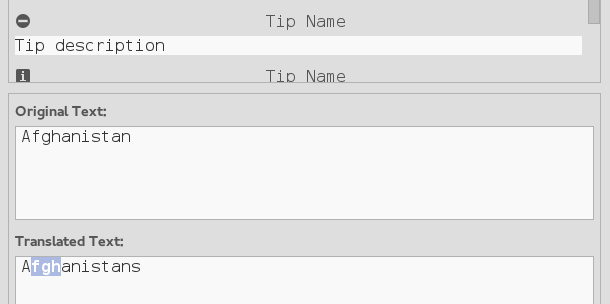
\includegraphics[width=0.6\textwidth]{img/selectedtip.png}
    \caption{Selección dun consello}
    \label{fig:ui:panel:edit:selectedtip}
\end{figure}

Desta forma cada columna amosará o nome do \lstinline{Tip} e o seu nivel de gravidade. O nome do consello debe ser suficiente para que o usuario se de conta do erro ao que se refire o consello. En caso de non ser suficiente o usuario pode premer encima do consello nese caso amosarase a descrición do consello e resaltarase a parte do texto á que refire o mesmo. Na Figura~\ref{fig:ui:panel:edit:selectedtip} podes mover ver unha captura desta situación.

Os cadros que permiten ver a cadeda orixinal están construídos co widget \lstinline{GTK.SourceView} este widget que non é parte da librería GTK extende o widget GTK.TextView e permite facer de forma sinxela, desfacer e refacer accións, resaltado de sintaxe e resaltado de espacios en blanco entre outros. Na Figura~\ref{fig:ui:panel:edit:pluralbox} podemos ver unha cadea con resaltado de sintaxe e de espazos en branco.

\begin{figure}[h!]
    \centering
    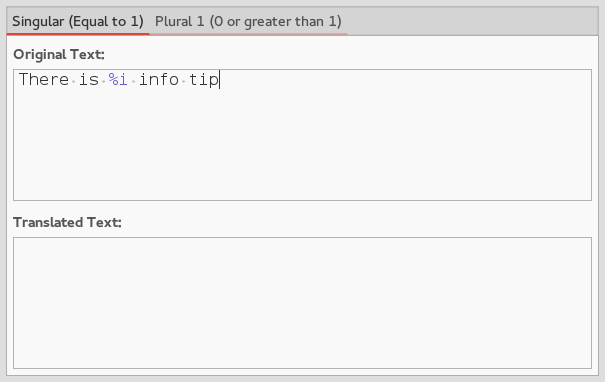
\includegraphics[width=0.6\textwidth]{img/editbox.png}
    \caption{Cadro de edición de mensaxes con plurais}
    \label{fig:ui:panel:edit:pluralbox}
\end{figure}

No caso de que a mensaxes a traducir teña plurais amosaremos cada plural nunha lapela. Como se pode ver na Figura~\ref{fig:ui:panel:edit:pluralbox}, no texto que amosa a lapela, aparte do número de plural amosaremos unha etiqueta explicando a que números se refire ese plural.

Debaixo do cadro de texto que amosa o contexto, temos botóns para ver as orixes da mensaxe actual e para cambiar o estado da mensaxe entre traducida e difusa. Para ver as orixes tamén se usa un widget \lstinline{GTK.Popover}.

A barra de tarefas ten botóns para volver a lista de ficheiros, gardar o ficheiro actual, facer e desfacer as accións, buscar, navegar a través do documento e ver as preferencias. Os botóns de volver a lista de ficheiros e de gardar son intercambiables de forma que so un deles se amosa en cada momento. Se o ficheiro foi modificado o botón que se amosa e o de gardar. Desta forma para ir a lista de ficheiros gardados deberemos salvar os cambios.


\subsubsection{Panel de Preferencias}
O panel de preferencias permite modificar como se algunhas opcións do programa, manexar os perfiles e activar ou desactivar plugins. Como podemos ver nas capturas da Figura~\ref{fig:ui:panel:preferences} temos tres pantallas para modificar as preferencias do programa.

\begin{figure}[h!]
  \centering
  \begin{subfigure}[b]{0.56\textwidth}
    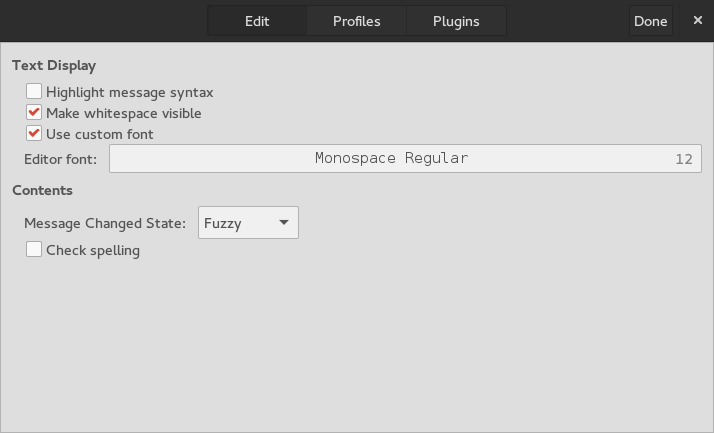
\includegraphics[width=\textwidth]{img/panel_preferencias_edicion.png}
    \caption{Edición}
  \end{subfigure}
  \begin{subfigure}[b]{0.56\textwidth}
    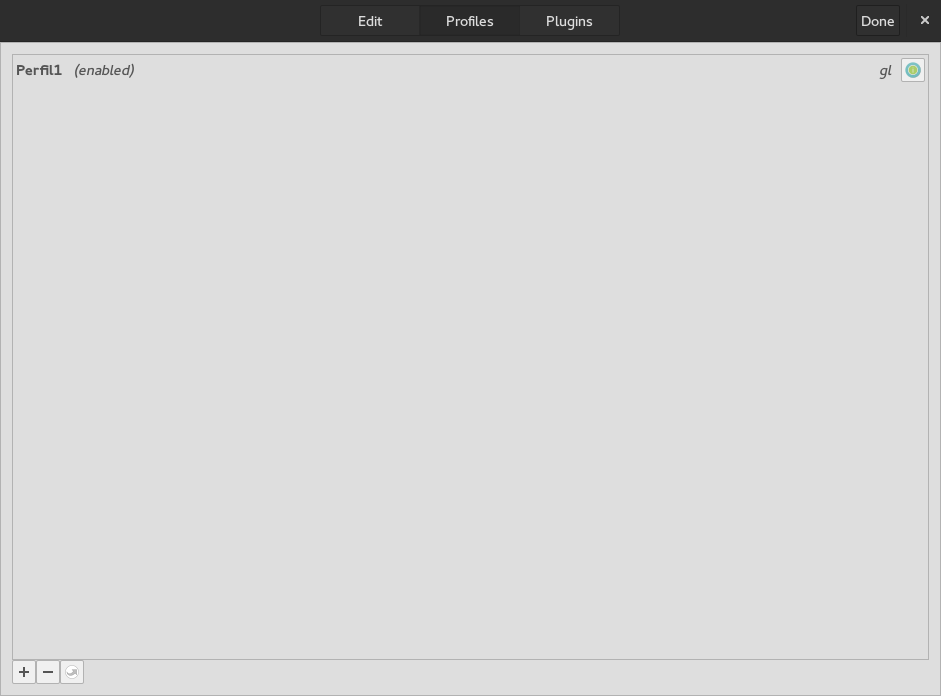
\includegraphics[width=\textwidth]{img/panel_preferencias_perfiles.png}
    \caption{Perfiles}
  \end{subfigure}
  \begin{subfigure}[b]{0.56\textwidth}
    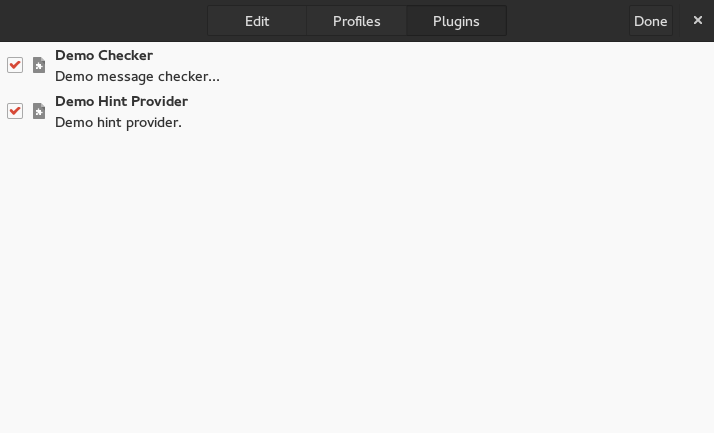
\includegraphics[width=\textwidth]{img/panel_preferencias_plugins.png}
    \caption{Plugins}
  \end{subfigure}
    \caption{Partes do panel preferencias}
    \label{fig:ui:panel:preferences}
\end{figure}

Navegamos entre estas tres pantallas empregando un widget \lstinline{GTK.StackSwitcher} incrustado na barra de ferramentas.

A pantalla de edición permite modificar o tipo de letra de algunhas partes do programa, o uso de resaltado de sintaxe ou o de espazos en branco. Ademais permite establecer cal é o estado ao que pasa unha cadea cando se traduce. O panel de perfil permite ver os perfiles existentes crear novos perfiles a través do panel de perfil, modificalos, eliminalos e activalos. Por último ca pantalla de plugins podemos ver a lista de plugins existentes e activalos ou desactivalos.


\subsubsection{Panel de Perfil}
O panel perfil permite a creación e modificación de perfiles. Esta dividido en dous subpaneis, un cos datos básicos do perfil e outro con datos avanzados. Estes dous paneis pódense ver na Figura~\ref{fig:ui:panel:profile}.
\begin{figure}[h!]
  \centering
  \begin{subfigure}[b]{0.5\textwidth}
    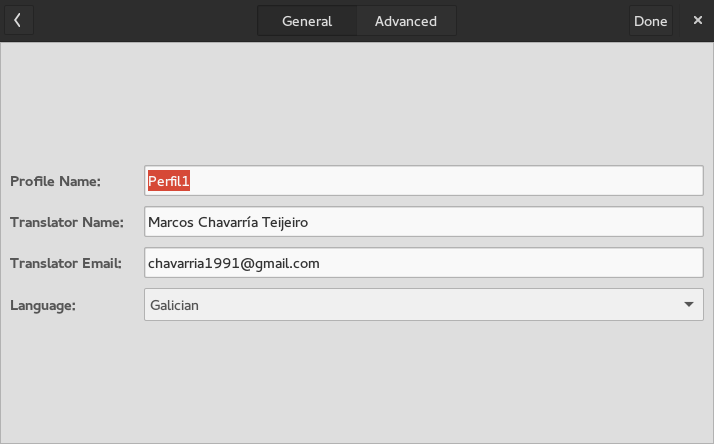
\includegraphics[width=\textwidth]{img/panel_pefil_xeral.png}
    \caption{Opcións básicas}
  \end{subfigure}
  \begin{subfigure}[b]{0.5\textwidth}
    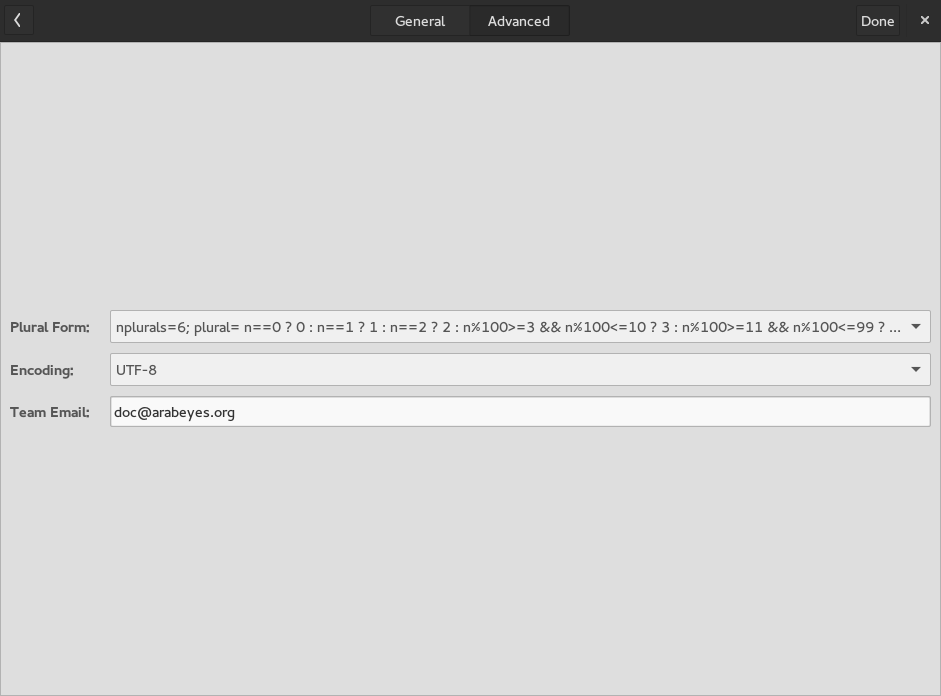
\includegraphics[width=\textwidth]{img/panel_perfil_avanzado.png}
    \caption{Opcións Avanzadas}
  \end{subfigure}
    \caption{Panel de perfil}
    \label{fig:ui:panel:profile}
\end{figure}

Esta división intenta mellorar a experiencia de usuario pois os valores avanzados autocompletanse cos valores por defecto no momento no que se selecciona a linguaxe.

\section{Navegación e Busca a través do documento}

Unha das partes importantes para facilitar a usabilidade da aplicación é que esta permita que o tradutor navegue polo ficheiro e busque termos de forma sinxela e rápida. Para facer isto creamos a clase abstracta \lstinline{Navigator}. Esta clase ten métodos sen argumentos que permiten avanzar ao seguinte, ao anterior, ao primeiro ou ao último elemento. O valor de volta destes métodos é un valor booleano que indica se esta operación foi posible.

\begin{figure}[h!]
  \centering
  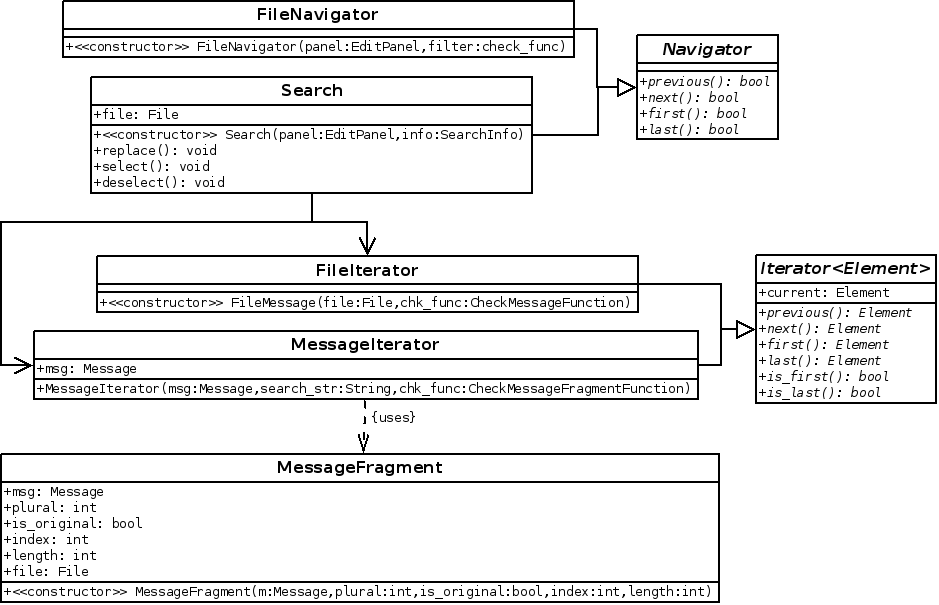
\includegraphics[width=\textwidth]{img/navigator_diagram.png}
  \caption{Diagrama de Clases de Navegación e Busca}
  \label{fig:nav:diagram}
\end{figure}

Para a implementación a busca dentro do documento creamos a clase \lstinline{Search}. Para implementar os métodos para avanzar a través dos resultados da busca empregamos dous iteradores, un que itera dentro dos mensaxes que cumpren os criterios e outro que itera dentro dos fragmentos das mensaxes.

Como podemos ver na Figura~\ref{fig:nav:diagram} os iteradores teñen métodos para conseguir o elemento actual, o primeiro, o último, o seguinte e o anterior. Ademais incorporan metodos para comprobar se o elemento actual é o último ou o primeiro.

As buscas permiten especificar o estado das mensaxes que queremos buscar e se o texto de busca está na cadea orixinal ou na traducida e se está na forma singular ou na plural. esta forma cando se inicia unha busqueda crease un iterador de ficheiro que itera entre os mensaxes que cumpren os requisitos e por cada mensaxe que cumpra os requisitos creamos un iterador de mensaxe que iterará devolvendo os fragmentos de mensaxe que cumpran os requisitos. Un \lstinline{MessageFragment} inclúe unha mensaxe, a forma plural do fragmento, se o fragmento está na cadea orixinal ou na tradución e o índice e lonxitude do fragmento.

Para seleccionar un fragmento da busca empregamos o método \lstinline{select()} do panel de edición.

En canto a implementación da navegación entre ficheiros a clase FileNavigator empregouse os métodos propios do widget TreeView de GTK. Créanse catro navegadores deste tipo un para as cadeas traducidas, outro para as cadeas sen traducir, outro para as cadeas con tradución difusa e outro para calquera cadea.

\section{Preferencias}
Necesitamos almacenar certas opcións do programa como pode ser o tipo e tamaño da letra a empregar ou se facemos resaltado e sintaxe. Para gardar toda esta información e que este dispoñible entre diferentes sesións do programa empregamos GSettings. GSettings é unha API para a xestión de configuración que forma parte do modulo GIO (GNOME Input/Output) dentro de GLib.

GSettings prové de métodos para obter e almacenar valores a partir dunha clave. Para almacenar estes valores soporta varios sistemas. Nós en concreto usamos o estándar en GNOME, \emph{dconf}. Este sistema está altamente optimizado para facer lecturas (o caso de uso máis habitual) de valores de configuración. Para usar GSettings debemos crear un ficheiro coas claves e tipos dos valores que imos empregar. No Fragmento de Código~\ref{lst:gsettings} podemos ver unha parte deste ficheiro.

\begin{lstlisting}[language=XML,label=lst:gsettings,caption=Fragmento da dos esquemas creados de GSettings]
<?xml version="1.0" encoding="UTF-8"?>
<schemalist>
  <schema path="/org/gnome/gnomecat/editor/" id="org.gnome.gnomecat.Editor">
    <key name="custom-font" type="b">
      <default>true</default>
      <summary>Use custom font.</summary>
      <description></description>
    </key>
    <key name="message-changed-state" type="s">
      <choices>
        <choice value='fuzzy'/>
        <choice value='translated'/>
      </choices>
      <default>'fuzzy'</default>
      <summary>Message Changed State</summary>
      <description>The state to set when a message is translated.</description>
    </key>
    [...]
  </schema>
  [...]
</schemalist>
\end{lstlisting}

Este ficheiro temos que compilalo e instalalo cas ferramentas que nos dá o módulo. Unha vez instalado obtemos unha instancia da clase GSettings que emprega o patrón Singleton e usamos esta instancia para obter e almacenar os valores.

Unha das vantaxes de GSettings é que permite enlazar unha propiedade dun obxecto de GObject con un valor de GSettings de forma que se modificamos o valor dun dos dous o outro vese reflexado. Empregamos esta característica para implementar a interface de preferencias na nosa aplicación de forma sinxela.

\subsection{Módulo de Perfiles}
Como vimos anteriormente ao falar da interface gráfica, os perfiles permiten configurar o nome e email co que se gardan os ficheiros e a linguaxe actual. Aínda que poden existir varios perfiles gardados so un estará activo en cada momento. Para almacenar estes perfiles tamén empregaremos GSettings.

\section{Plugins}
Os plugins permiten estender o programa engadíndolle funcionalidade. Dous dos puntos máis sinxelos para engadir funcionalidade son as pistas e os consellos. Estes dous elementos que están pensados para axudar os tradutores son aportados polos plugins. Existen dúas sinais de nomes \lstinline{check_message} e \lstinline{provide_hints} que son usadas para crear instancias de pistas e de consellos. Estas sinais son chamadas dende os plugins.

Para implementar estes plugins empregamos a biblioteca \emph{LibPeas}. Esta biblioteca foi creada para poder incluír extensións en GEdit, o editor de texto de GNOME. Trátase dun motor de plugins baseado en GObject. Permite a carga de plugins en varios linguaxes de programación como Vala, C, Python ou JavaScript.

Os plugins son unha unidade de compilación diferente ao programa principal. Para que desde esta unidade independente de compilación coñeza parte da API creada para ficheiros, perfiles e linguaxes debemos incluír estes ficheiros tamén nesta unidade de compilación. Creamos ademais unha pequena interface que inclúe as dúas sinais que citamos anteriormente. Esta interface é implementada pola clase aplicación.

A biblioteca LibPeas emprega o patrón Singleton para darnos unha instancia dun motor de plugins. A este motor temos que indicarlle a ruta do sistema onde ten que buscar os plugins e cargar os plugins que atopen. Ademais cargamos un obxecto de clase

Para implementar un plugin temos que crear dous ficheiros. O primeiro ficheiro contén no nome do plugin información sobre o plugin como a descrición, o autor ou autores e o Copyright. No Fragmento de Código~\ref{lst:plugin:metadata} pódese ver un exemplo deste ficheiro.

\begin{lstlisting}[label=lst:plugin:metadata,caption=Ficheiro de metadatos do plugin]
[Plugin]
Module=demochecker
Name=Demo Checker
Description=Demo message checker...
Authors=Marcos Chavarría Teijeiro <chavarria1991@gmail.com>
Copyright=Copyright (C) 2014 Marcos Chavarría Teijeiro
\end{lstlisting}

O outro ficheiro é a implementación do propio plugin. Debemos implementar unha ou máis extensións e unha función onde as rexistraremos. A función ten que ter o nome \lstinline{peas_register_types()} e usará a etiqueta \lstinline{ModuleInit} de forma que se executará cando se inicialice o módulo.

\begin{lstlisting}[label=lst:plugin:code,caption=Fragmento da implementación do plugin DemoChecker]
public class DemoChecker : Peas.ExtensionBase,  Peas.Activatable
{
    public Object object  { owned get; construct; }

    public void activate ()
    {
      (object as GNOMECAT.API).check_message.connect (on_check_message);
    }

    public void deactivate ()
    {
      (object as GNOMECAT.API).check_message.disconnect (on_check_message);
    }

    public void update_state ()
    {
    }

    [...]
}

[ModuleInit]
public void peas_register_types (GLib.TypeModule module)
{
  var objmodule = module as Peas.ObjectModule;
  objmodule.register_extension_type (typeof (Peas.Activatable),
                                     typeof (DemoPlugins.DemoChecker));
}
\end{lstlisting}

Para implementar unha extensión temos que implementar unha clase que implemente a interface Activable e herede da clase ExtensionBase. A interface Activable inclúe os métodos que se executarán cando se active e desactive o plugin. No Fragmento de Código~\ref{lst:plugin:code} amosase parte do código empregado para o plugin de exemplo \emph{DemoPlugin}. Podemos ver como nos métodos para activar e desactivar conectamos e desconectamos a sinal \lstinline{check_message} para poder xerar os Tips de exemplo.

